\section{Publications}
\label{sec:publications}

The following Sections list the works published and presented during the accomplishment of this Thesis. When identified with a $^{\dagger}$, the authors contributed equally to the publication work.

In addition, Figure \ref{fig:timeline} illustrates the timeline of publications, presentations and research stays of this Thesis.

\begin{figure}
    \centering
    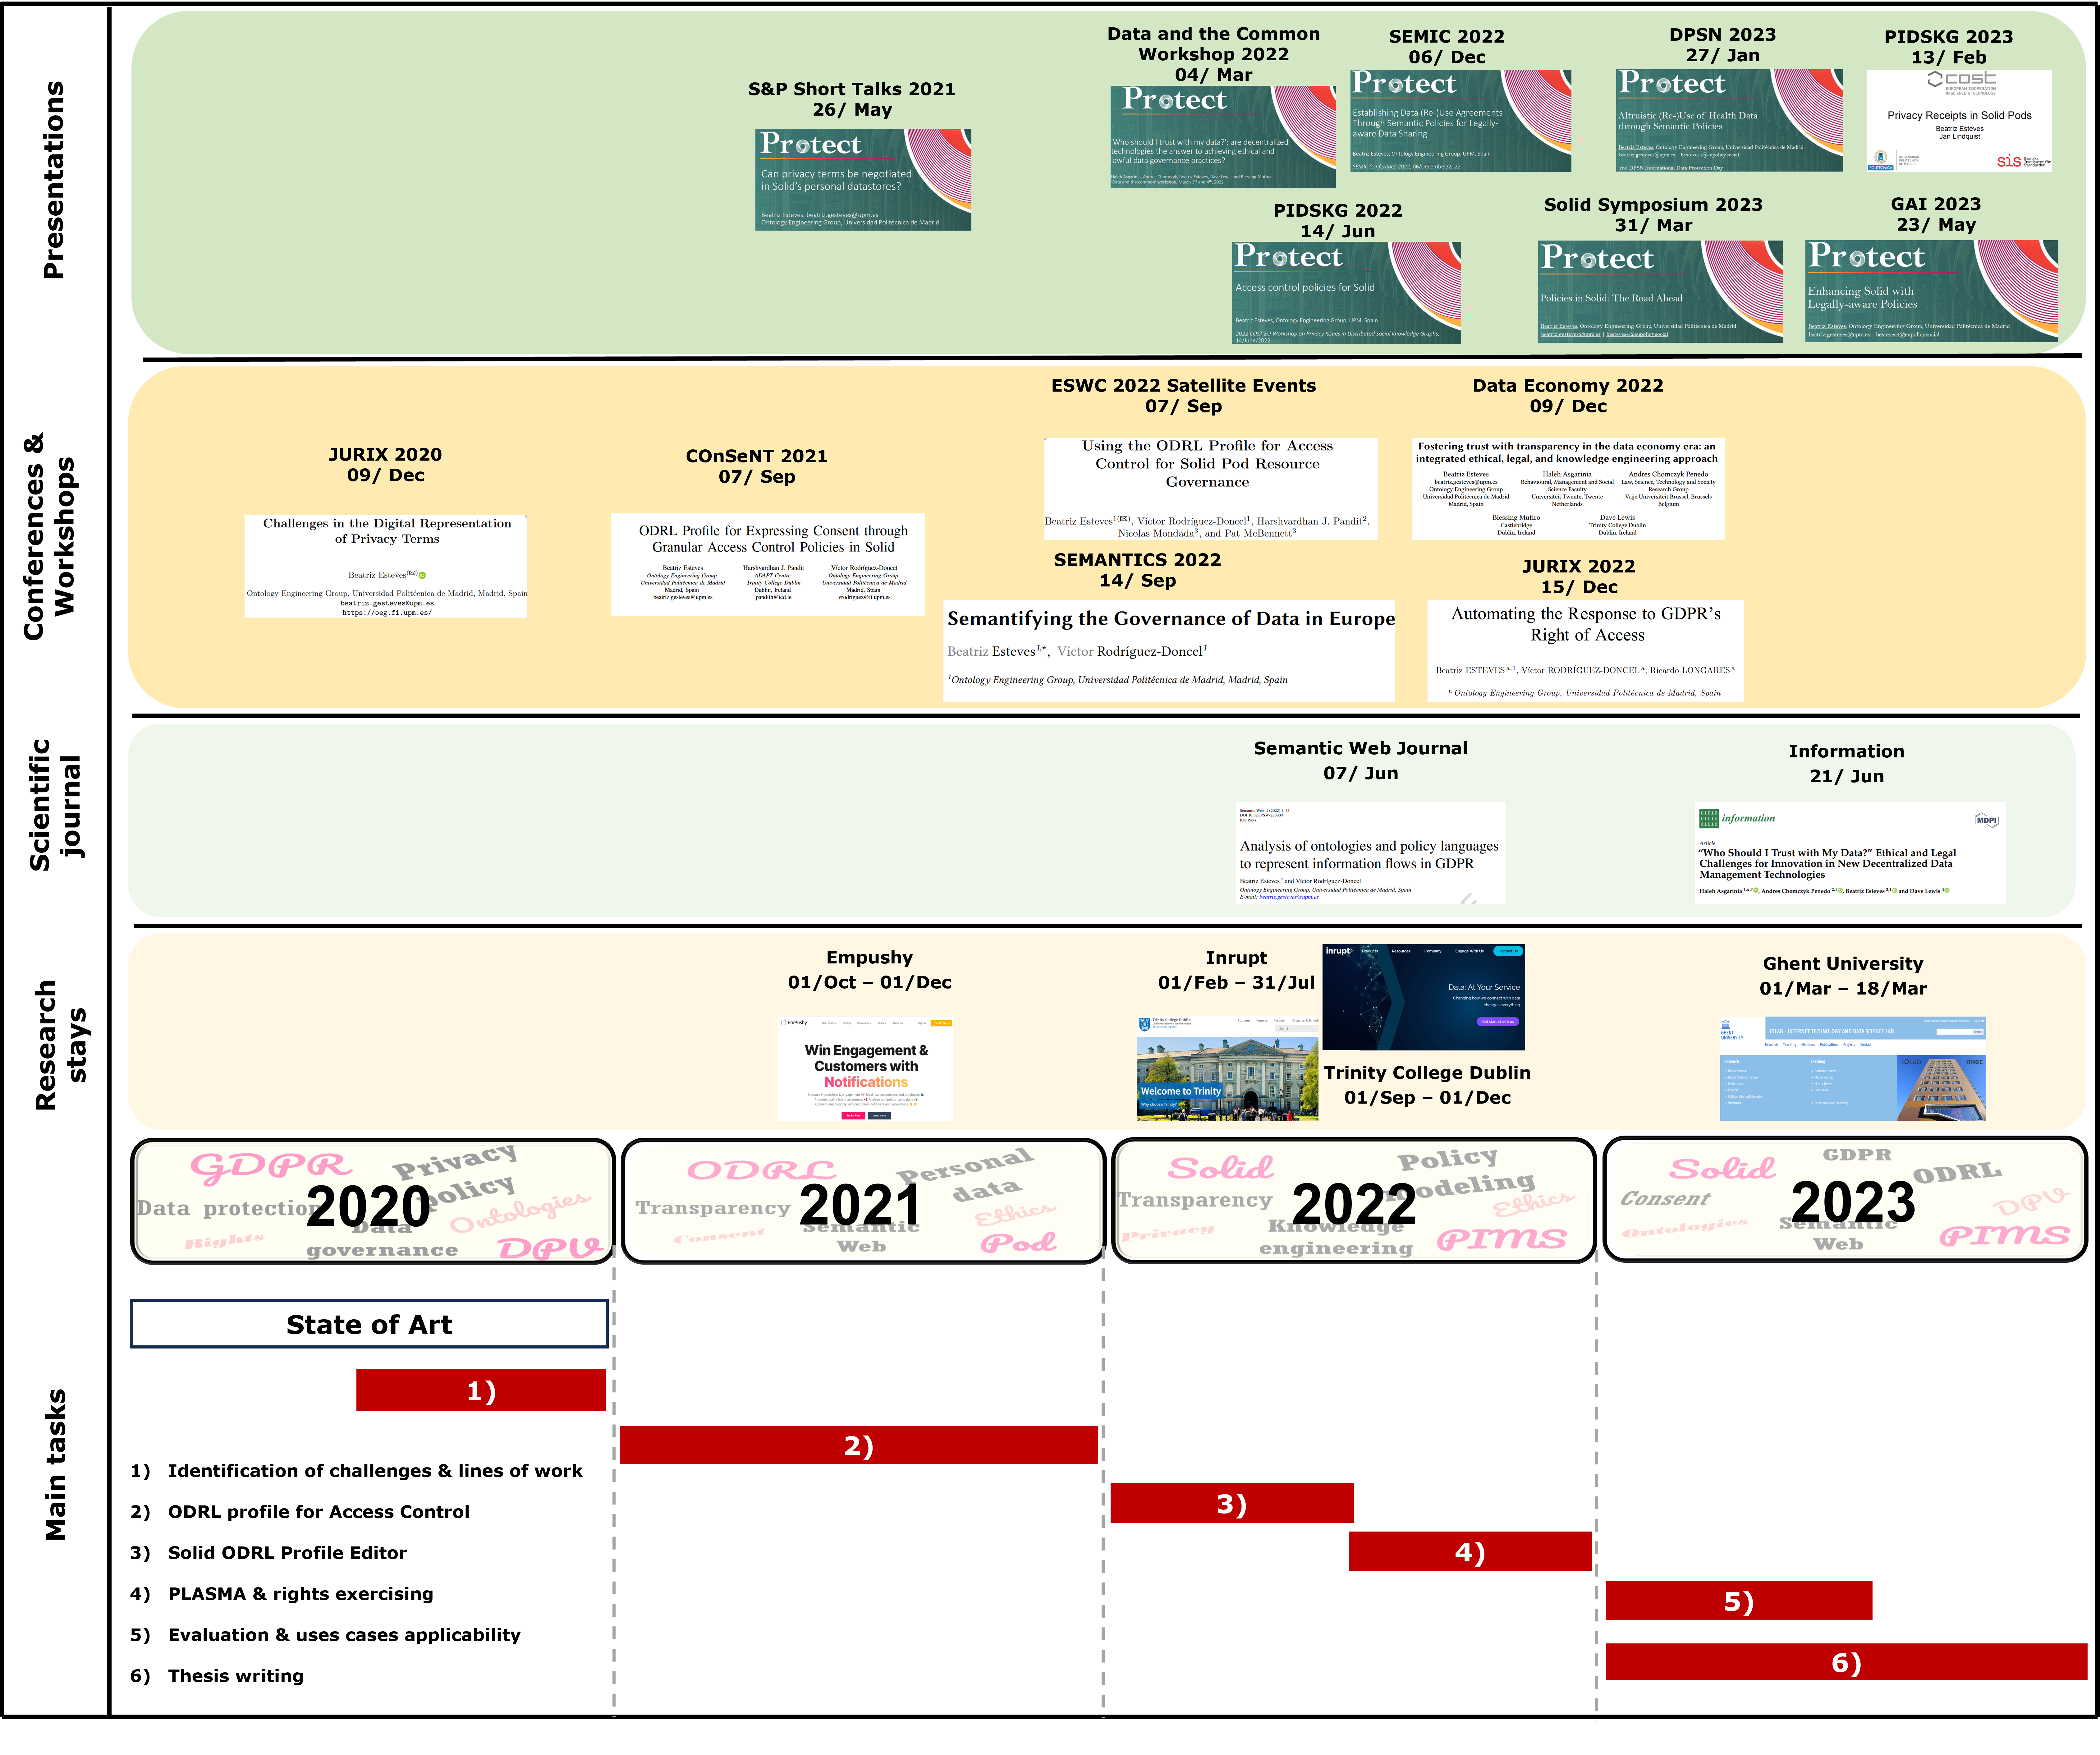
\includegraphics[width=\linewidth]{figures/chapter-1/timeline.png}
    \caption{Timeline of publications, presentations and research stays of this Thesis.}
    \label{fig:timeline}
\end{figure}

\subsection{Journal contributions}
\label{sec:publications_journal}

\begin{enumerate}
    \item [(PJ1)] Analysis of Ontologies and Policy Languages to Represent Information Flows in GDPR. (2022) \textbf{B. Esteves}, V. Rodríguez-Doncel. \textit{Semantic Web Journal}, pp. 1--35. \beatriz{update when SWJ issue is published}
    \item [(PJ2)] ``Who Should I Trust with My Data?'' Ethical and Legal Challenges for Innovation in New Decentralized Data Management Technologies. (2023) H. Asgarinia$^{\dagger}$, A. Chomczyk Penedo$^{\dagger}$, \textbf{B. Esteves}$^{\dagger}$, D. Lewis. \textit{Information 14(7)}, \url{https://doi.org/10.3390/info14070351}.
\end{enumerate}

\subsection{Conference contributions}
\label{sec:publications_conference}

\begin{enumerate}
    \item [(PC1)] Extracting and Understanding Call-to-actions of Push-Notifications. (2022) \textbf{B. Esteves}, K. Fraser, S. Kulkarni, O. Conlan, V. Rodríguez-Doncel.  In \textit{Natural Language Processing and Information Systems. Edited by P. Rosso, V. Basile, R. Martínez, E. Métais, F. Meziane, Volume 13286}, pp. 147-–159. Springer International Publishing. \url{https://doi.org/10.1007/978-3-031-08473-7\_14}.
    \item [(PC2)] Now, Later, Never: A Study of Urgency in Mobile Push-Notifications. (2022) \textbf{B. Esteves}, K. Fraser, S. Kulkarni, O. Conlan, V. Rodríguez-Doncel. In \textit{Advances in Mobile Computing and Multimedia Intelligence. Edited by P. Delir Haghighi, I. Khalil, G. Kotsis}, pp. 38-–44. Springer Nature Switzerland. \url{https://doi.org/10.1007/978-3-031-20436-4\_4}.
    \item [(PC3)] Automating the Response to GDPR’s Right of Access. (2022) \textbf{B. Esteves}, V. Rodríguez-Doncel, R. Longares. In \textit{Legal Knowledge and Information Systems}, pp. 170–-175. IOS Press. \url{https://doi.org/10.3233/FAIA220462}.
    \item [(PC4)] Semantics for Implementing Data Reuse and Altruism Under EU’s Data Governance Act. (2023) \textbf{B. Esteves}, V. Rodríguez-Doncel,  H. J. Pandit, D. Lewis. In \textit{Knowledge Graphs: Semantics, Machine Learning, and Languages. Edited by M. Acosta et al.}, pp. 210--226. IOS Press. \url{https://doi.org/10.3233/SSW230015}.
\end{enumerate}

\subsection{Workshop contributions}
\label{sec:publications_workshop}

\begin{enumerate}
    \item [(PW1)] Challenges in the Digital Representation of Privacy Terms. (2021) \textbf{B. Esteves}. In \textit{AI Approaches to the Complexity of Legal Systems XI-XII. Edited by V. Rodríguez-Doncel, M. Palmirani, M. Araszkiewicz, P. Casanovas, U. Pagallo, G. Sartor, Volume 13048}, pp. 313–-327. Springer International Publishing. \url{https://doi.org/10.1007/978-3-030-89811-3\_22}.
    \item [(PW2)] ODRL Profile for Expressing Consent through Granular Access Control Policies in Solid. (2021) \textbf{B. Esteves}, H. J. Pandit, V. Rodríguez-Doncel. In \textit{2021 IEEE European Symposium on Security and Privacy Workshops (EuroS\&PW)}, pp. 298-–306. \url{https://doi.org/10.1109/EuroSPW54576.2021.00038}
    \item [(PW3)] Using the ODRL Profile for Access Control for Solid Pod Resource Governance. (2022) \textbf{B. Esteves}, V. Rodríguez-Doncel, H. J. Pandit, N. Mondada, P. McBennett. In \textit{The Semantic Web: ESWC 2022 Satellite Events. Edited by P. Groth, A. Rula, J. Schneider, I. Tiddi, E. Simperl, P. Alexopoulos, R. Hoekstra, M. Alam, A. Dimou, M. Tamper}, pp. 16-–20. Springer International Publishing. \url{https://doi.org/10.1007/978-3-031-11609-4\_3}
    \item [(PW4)] Semantifying the Governance of Data in Europe. (2022) \textbf{B. Esteves}, V. Rodríguez-Doncel. In \textit{18th International Conference on Semantic Systems - CEUR Workshop Proceedings, Volume 3235}. \url{https://ceur-ws.org/Vol-3235/paper17.pdf}.
    \item [(PW5)] Fostering trust with transparency in the data economy era: An integrated ethical, legal, and knowledge engineering approach. (2022) \textbf{B. Esteves}, H. Asgarinia, A. Chomczyk Penedo, B. Mutiro, D. Lewis. In \textit{Proceedings of the 1st International Workshop on Data Economy}, pp. 57-–63. \url{https://doi.org/10.1145/3565011.3569061}.
    \item [(PW6)] Towards an Architecture for Data Altruism in Solid. (2023) \textbf{B. Esteves}. In \textit{22nd International Semantic Web Conference: Posters, Demos, and Industry Tracks}. (Accepted for publication)
    \item [(PW7)] Using Patterns to Manage Governance of Solid Apps. (2023) \textbf{B. Esteves}, H. J. Pandit. In \textit{14th Workshop on Ontology Design and Patterns (WOP 2023@ISWC 2023)}. (Accepted for publication)
\end{enumerate}

\subsection{Oral presentations}
\label{sec:oral_presentations}

The following presentations were given during the realisation of this Thesis.

\beatriz{create post with oral presentations with links to abstracts and slides of presentations in Zenodo}

\begin{enumerate}
    \item [(OP1)] Can privacy terms be negotiated in Solid's personal datastores? \textbf{B. Esteves}. Short talk at the \textit{2021 IEEE Symposium and Workshops on Security \& Privacy} (26/May/2021).
    \item [(OP2)] `Who should I trust with my data?': are decentralised technologies the answer to achieving ethical and lawful data governance practices? H. Asgarinia, A. Chomczyk Penedo, \textbf{B. Esteves}, D. Lewis, B. Mutiro. Presentation at the \textit{Data and the Common Workshop 2022} (04/March/2022).
    \item [(OP3)] Access control policies for Solid. \textbf{B. Esteves}. Demonstration at the \textit{2022 COST EU Workshop on Privacy Issues in Distributed Social Knowledge Graphs} (14/June/2022).
    \item [(OP4)] Establishing Data (Re-)Use Agreements Through Semantic Policies for Legally-aware Data Sharing. \textbf{B. Esteves}. Lightning talk at the \textit{SEMIC Conference 2022} (06/December/2022).
    \item [(OP5)] Altruistic (Re-)Use of Health Data through Semantic Policies. \textbf{B. Esteves}. Short talk at the \textit{2nd DPSN International Data Protection Day} (27/January/2023).
    \item [(OP6)] Privacy Receipts in Solid Pods. \textbf{B. Esteves}, J. Lindquist. Presentation at the \textit{2023 COST EU Workshop on Privacy Issues in Distributed Social Knowledge Graphs} (13/February/2023).
    \item [(OP7)] Policies in Solid: The Road Ahead. \textbf{B. Esteves}. Presentation at the \textit{Solid Symposium 2023} (31/March/2023).
    \item [(OP8)] Enhancing Solid with Legally-aware Policies. \textbf{B. Esteves}. Presentation at the \textit{Governing Artificial Intelligence International Symposium 2023} (23/May/2023).
\end{enumerate}

\subsection{Submitted contributions}
\label{sec:publications_submitted}

The following contributions are currently under review in different journals.

\begin{enumerate}
    \item [(PS1)] (UNDER REVIEW) Enhancing Data Use Ontology (DUO) for Health-Data Sharing by Extending it with ODRL and DPV. (2022) H. J. Pandit$^{\dagger}$, \textbf{B. Esteves}$^{\dagger}$.  \textit{Semantic Web Journal}.
    \item [(PS2)] (UNDER REVIEW) `I Consent to These Terms': A Legal and Technical Approach for Obtaining Valid Consent in Solid. (2023) M. Florea$^{\dagger}$, \textbf{B. Esteves}$^{\dagger}$. \textit{Special Issue on Addressing Privacy and Data Protection in New Technological Trends of the Information journal}.
\end{enumerate}